\documentclass[aps, rmp, 11pt, notitlepage]{revtex4-1}
\usepackage{graphicx}
\usepackage{subfigure}
\usepackage{amsmath}
\usepackage[bookmarks, hyperindex, colorlinks=true,
            linkcolor=red,
            urlcolor=blue, citecolor=blue]{hyperref}
   
\usepackage{listings}
\lstset{
  basicstyle=\ttfamily\footnotesize,
  showstringspaces=false,
  commentstyle=\color{Maroon},
  keywordstyle=\color{Blue},
  tabsize=4,
  frame=lines
}

\usepackage{bm}
\usepackage{mwe} 
\usepackage[usenames,dvipsnames,svgnames,table]{xcolor}

\def\comment#1{\textcolor{red}{#1}}
\renewcommand{\vec}[1]{\bm{#1}}

\renewcommand{\baselinestretch}{1.2}
\def\keywords#1{\textcolor{blue}{{\bf #1}}}
\def\function#1{\textcolor{blue}{{\it #1}}}
\usepackage[final]{changes}
\usepackage{changes}
\usepackage{lipsum}
\makeatletter

\graphicspath{{./figures/}}

\begin{document}
\title{Incorporating node-local storage in system-aware HDF5 VFD}
\author{Huihuo Zheng and Venkatram Vishwanath}
\date{\today}
\affiliation{
Argonne Leadership Computing Facility, 
\\ Argonne National Laboratory}
\date{January 29, 2020}
\begin{abstract}
Many high performance computing (HPC) clusters have two types of storage, a remote storage media of the global parallel file system such as Lustre or GPFS, and node-local storage attached to the compute nodes such as SSDs. 
To our knowledge, the node-local storage are rarely integrated into the parallel I/O workflows in real applications.
We present an approach to incorporate node-local storage as a cache to the parallel file system to ``effectively" improve the parallel I/O efficiency. This document outline the details of our prototype design and initial performance evaluation on Theta, a Cray X40 supercomputer at Argonne Leadership Computing Facility (ALCF). 
\end{abstract}
\maketitle
\section{Introduction}
\label{sec:intro}
Many high performance computing (HPC) clusters use a global parallel file system such as Lustre or GPFS for a high I/O throughput. The parallel file system storage are usually separated from the compute nodes. Data access thus involves transferring data from the global storage media to the compute nodes through the interconnect. Besides the remote storage, the compute nodes are often equipped with node-local storage such as SSDs. These node-local storage are only accessible during the simulation and each local storage device is visible only to those processes on the same node. Thus, it is not very straight forward to integrate the node-local storage into the I/O workflows. Very rare teams have made full usage of these local storage. 

We present here our prototype design of incorporating the node local storage into the parallel write and parallel read workflow. For parallel write workflow, the main design is to write the data to the node-local storage first, and then migrate the data to the parallel file system in an asynchronous way. We expect that there is compute work right after the I/O, therefore, the asynchronous data migration will most likely be hidden behind the compute work. Thus, outwardly, the I/O performance is determined by I/O bandwidth writing data to the node-local storage. 

For parallel read workflow, we focus on multiple repeated read workflow, such as deep learning workflow. In this case, in the first iteration, we read the data from the parallel filesystem, and then cache it to the node local storage in an asynchronous way. In the following iterations, we directly get data from the node local storage. In this way, we have the same performance for the first iteration whereas higher performance for the following up iterations.  

\section{Parallel write workflow}
In this milestone, we present an approach to integrate the local storage into the parallel I/O workflows by using them as a cache to the file system for data staging. For example, for write, rather than directly writing data from the memory to the parallel file system, we will first write them to the local storage and then move them from the local storage to the parallel file system in the background asynchronously without affect the rest of the simulation. The workflow is schematically shown in Fig.~\ref{fig:schematic}. From the application perspective, since the data migration from the local storage to the filesystem is on the background while the other part of the application is running, the only I/O cost is from writing data to the local storage devices, which is local and does not go through the interconnect. Therefore, writing data to the local storage devices is highly scalable without contention and typically has a much higher aggregate I/O rate. For example, on Theta, an XC40 system at ALCF, each node is attached with a SSD have a write rate approximately 500 MB. The aggregate write rate is 2 TB. This is much higher than the aggregate bandwidth from the Lustre file system which is about 200 GB. Therefore, by using node-local storage as a cache to stage the data effectively improve the parallel I/O throughput from the user perspective. 

\begin{figure}[hbt]
\centering
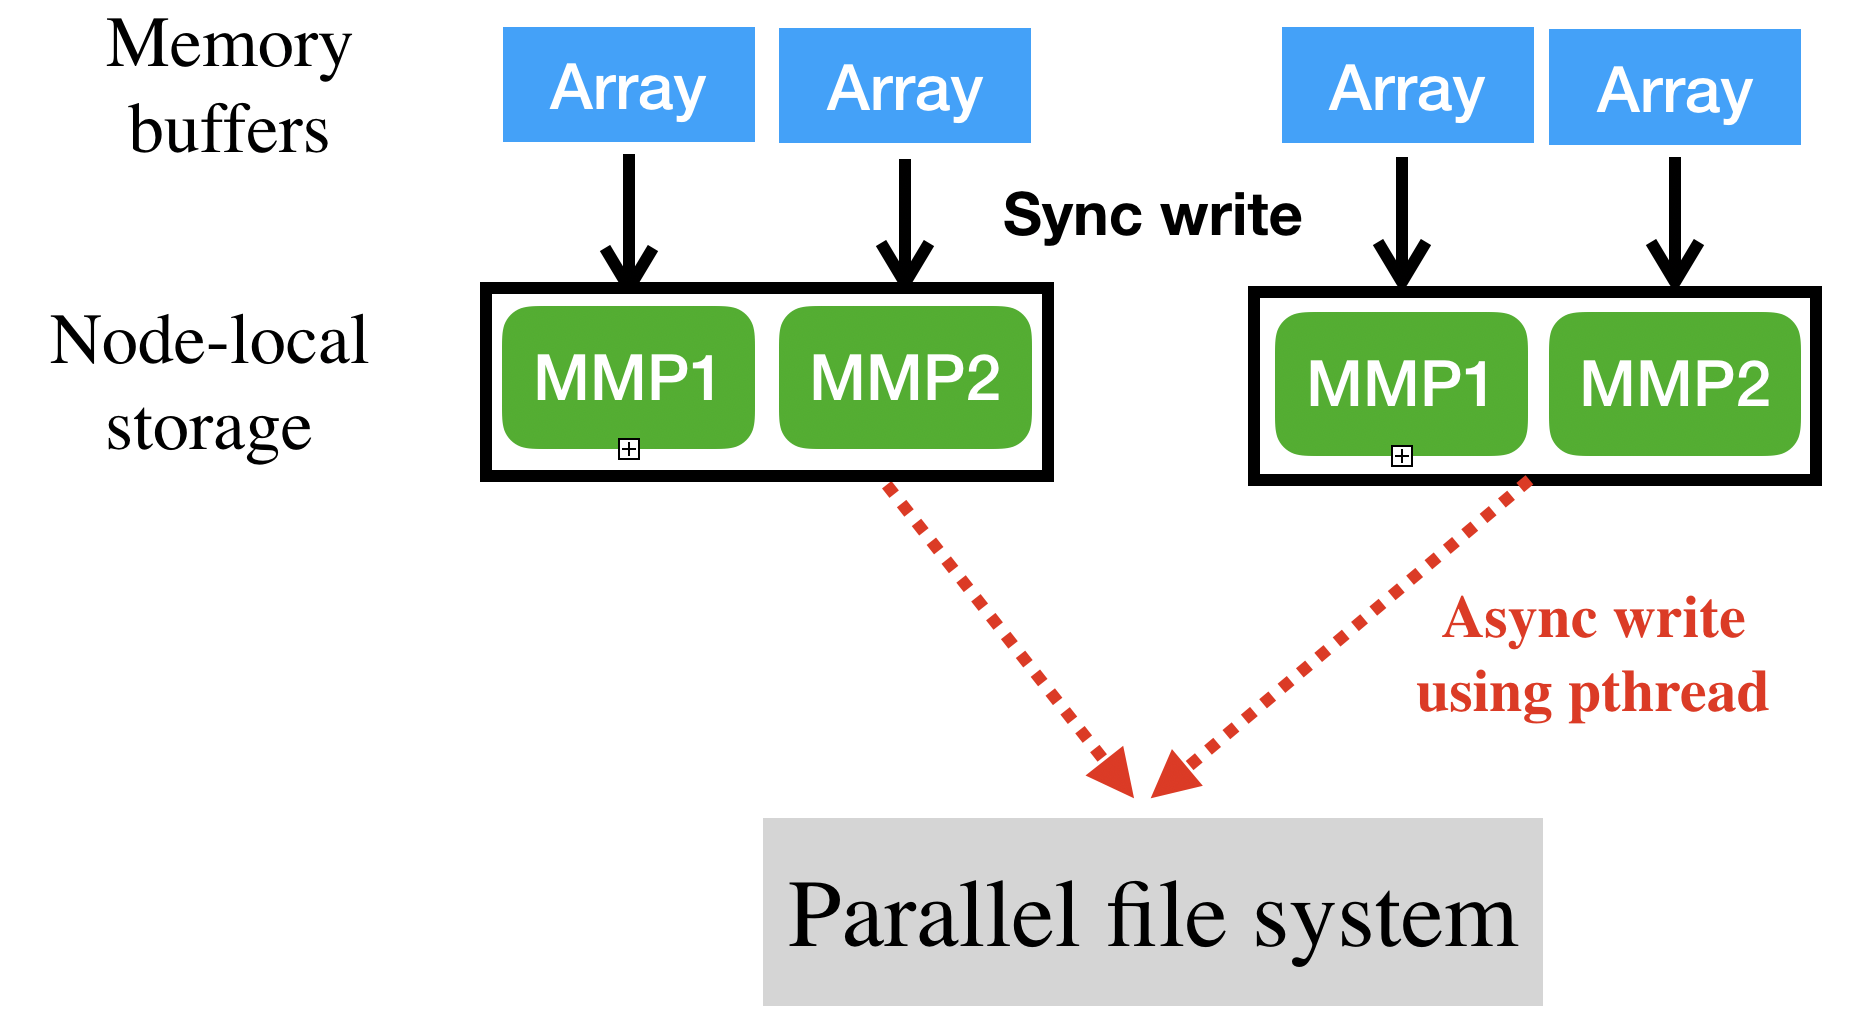
\includegraphics[width=0.6\textwidth]{schematic.png}
\caption{Schematic demonstration of incorporating node-local storage into the parallel I/O workflow. The memory buffers are written into the node-local storage first, and then migrated to the file system asynchronously by a pthread through parallel I/O function calls.}\label{fig:schematic}
\end{figure} 

The whole workflow is conceptually simple. However, it does need careful design to incorporate the workflow into I/O libraries such as MPI I/O and HDF5 such that it can be easily adopted by the application developers.  Ideally, the application developers shall not need to be aware of the underneath I/O process. They should make minimal change or even no change to their code to adopt this framework. In Sec.~\ref{sec:design}, we will provide the details of our prototype design in both MPI I/O and system-aware HDF5 library to meet all these needs. In Sec.~\ref{sec:design}, we then provide our initial performance evaluation on Theta and discuss our future work to fully integrate into the VFD framework in the HDF5 library. 

\subsection{Prototype design}
\label{sec:design}
\subsubsection{Design choices}
In order to make sure that this framework can be widely adopted by application developers, and at the same time, easily integrated into other functionality of the I/O library, such as topology-aware data aggregation, we have the following considerations: 
\begin{itemize}
\item [(1)] Application developers need no change or only minimal change to their code in order to use the local-storage caching /staging feature. In order to achieve this, we shall use the same top level API / function calls and modify the underneath implementation. For example, in MPI I/O, this can be achieved by inserting local-storage operations in between the high level MPI I/O calls and the low level PMPI I/O calls.

\item [(2)] From the user perspective, the I/O calls shall look like blocking I/O calls outwardly. In other words, the buffer should be usable and modifiable right after the I/O function returns. Therefore, the async process shall be hidden underneath to execute the data migration after the I/O function returns.  

\item [(3)] We shall guarantee all the data being pushed to the file system before closing the file. In other words, the program shall wait until all the I/O tasks are finished before MPI\_File\_close / H5Fclose is called. 

\item [(4)] Ideally, we shall no introduce extra memory usage. This can be achieved by using memory mapped file on the local storage, so that we do not need to allocate extra memory to the buffer for the data migration.
\end{itemize}

Regarding the asynchronous data migration from the local storage to the parallel file system, we can potentially use nonblocking I/O calls or use a helper thread such as pthread to perform data migration. We choose the latter for the following reasons: (a) nonblocking I/O calls might not always be supported in the system; (b) even if it is supported, other parts of the HDF5 library might already uses nonblocking I/O. For example, in the topology-aware HDF5 VFD, non-blocking I/O functions are used to overlap the data aggregation with parallel I/O. In such case, It will be difficult to integrate the async data migration into the topology-aware VFD. On the contrary, using pthread allows us to perform async I/O at a high level, independent of underneath implementation of the corresponding parallel I/O function. One particular feature about pthread is that it can create another pthread by itself. Even if the I/O function from the library already uses pthread underneath, one can use pthread to execute that function and extra pthread will be created as needed. The only drawback is that creating pthread will use extra hardware resource. This will not be a problem as more and more HPC platforms are heterogeneous. The majority of the compute works will presumably be offloaded into the accelerators. Therefore, allocating one thread on the host to perform I/O shall not degrade the performance of the application. 

%We create a global pthread to execute the high level I/O function, such as MPI\_File\_write\_... in MPI I/O or H5Dwrite in HDF5. 
\subsubsection{Function API}
Currently, in the prototype implementation, we create H5Fcreate\_cache, H5Dwrite\_cache, and H5Fclose\_cache functions to replace H5Fcreate, H5Dwrite, and H5Fclose. The implementation of the three *\_cache functions are as follows: 
\begin{itemize}
\item H5Fcreate\_cache: we perform the following three major things: each rank create a file on the local storage; creating a pthread and put it into sleep first; calling H5Fcreate to create a HDF5 file on the file system and returning the file handle. 
\item H5Dwrite\_cache: we write the memory buffer to the file on the local storage in appending mode, and adding an I/O task to the task list. Each I/O task contains arguments for the pthread function. We wake up the I/O pthread to execute the async I/O when the number of unfinished tasks is not zero. pthread will then pick a task from the list and create a memory map to the file with an offset, and execute H5Dwrite to write the mmap buffer to the file system. We check whether the space left on the SSD is enough for writing the memory buffer. If not, we put a conditional wait on the master thread to wait until previous I/O tasks finished and then write the buffer to the beginning of the file on the local storage. 
\item H5Fclose\_cache: in this function, we put a conditional wait for the master threads to wait until all the I/O tasks are finished. We then perform H5Fclose to close the remote HDF5 file on the file system and remove all the temporal files on the local storage. We then join the pthread with the master pthread and release the resources associated to the pthread. 
\end{itemize}
Besides, we also created H5Dclose\_cache, H5Pclose\_cache, in which we add a conditional wait to the master thread to wait for the pthread to finish all the I/O tasks before closing the dataset or the property lists. 

All these XXX\_cache functions are used only in this prototype design. In future, we will use the same APIs and the caching function can be enabled by setting environmental variables, so that the application developers do not need to modify their code. This approach is very straightforward. Another potential approach is to incorporate the caching into MPI I/O file transfer property list and the cache functionality will be enabled at the low level VFD instead of at the H5Dwrite level. However, the latter approach might need more efforts to make it compatible with the rest of the HDF5 library. 
\subsubsection{Using local storage cache}
Finally, in real applications, in order to gain benefit from this local-storage implementation,  one should insert enough compute work between the H5Dwrite\_cache call and the H5Fclose\_cache call such as 
\begin{lstlisting}
for(int iter=0; iter < nw; nw++)
	... # other works before I/O
	H5Fcreate_cache()
	H5Dwrite_cache()
	... # compute works to overlap with the data migration
	H5Fclose_cache()
}
\end{lstlisting}
or 
\begin{lstlisting}
H5Fcreate_cache()
for(int iw=0; iw < nw; nw++)
	... # some works before I/O
	H5Dwrite_cache()
	... # compute works to overlap with the data migration
}
H5Fclose_cache()
\end{lstlisting}

Then environmental variable \textbf{SSD\_CACHE\_PATH} is used to inform the library the path of the node-local storage. By default, it is set to be /local/scratch. Currently, the capacity of the storage is hard coded to be 128 GB. This can be modified in H5SSD.c. 

The source code and the benchmarks code for the prototype design are located in \\https://xgitlab.cels.anl.gov/ExaHDF5/node\_local\_storage.git. This TeX source code of this document is included in the ./doc folder in the git repository. 
\subsection{Initial performance evaluation}


We carried initial performance evaluations for node-local-storage caching. We put sleep in between H5Dwrite\_cache() and H5Fclose\_cache() to mimic computation in the application, we then measure the time spent on H5Dwrite\_cache and calculate the write rate. We perform the evaluation on Theta. The dimension of the local memory space on each rank is $(2048, 2048)$. The dimension of the file space is $(2048\times np\times nw, 2048)$, where $np$ is the number of MPI processes, $nw$ is the number of write. The data is transferred from memory space to the file space through collective MPI I/O. The Lustre stripe setting is stripe count = 48, and stripe size = 16 MB. 

\begin{table}[hbt]
\centering
\caption{Time (in second) spent on write and close for different amount of compute. The buffer size is 16 MB. The test is done on 8 KNL nodes, with 32 processes per node. }\label{tab:async}
\begin{tabular}{l||cccccc}
\hline
Run & 1 & 2 & 3 & 4 & 5 & 6 \\
\hline
\hline
Compute     & 0.03 &  0.34 & 0.64 & 0.91 & 1.21  & 2.02\\
H5Dwrite\_cache &  0.95 & 0.94 & 0.93 &  0.95 & 0.95  & 0.94 \\
H5DFclose\_cache & 0.97  & 0.68 & 0.36 & 0.06 & 0.08 & 0.07\\ 
\hline
\hline
Total & 1.95  & 1.96 & 1.93 & 1.92 & 2.24 & 3.03 \\
\hline
\end{tabular}
\end{table}
We first test the async feature of the implemation. Without inserting compute in between H5Dwrite\_cache and H5Fclose\_cache. The data migration will mostly manifest in H5Fclose\_cache. As we increase the amount of compute, more and more portion of data migration will overlap with compute, and the time for H5Fclose\_cache shall reduce. We perform such a test on 8 nodes, with 32 ranks per node. The local buffer size is set to be 16 MB, and $nw=1$. This is shown in Table~\ref{tab:async}. The time for data migration is about 1.0 second. If the compute is more than 1.0 second, the data migration will be completely hidden. 


Next we text the overall ``effective" I/O rate for SSD cache HDF5. We assume that the amount of compute is enough to overlap with the data migration. Therefore, we measure the time spent in H5Dwrite\_cache and compute the ``effective" I/O rate appeared to the application. We compare it with the I/O rate using H5Dwrite to write directly to the file system. The results are shown in Fig.~\ref{fig:perf}.
 As we can see, without SSD cache, the write rate saturated at about 10 GB/sec. With SSD cache, since the collective write happens in the background, the I/O cost is purely from writing to SSDs. It scales linearly with respect to the number of nodes as we expected. For the case of 512 nodes, it reaches 250 GB/sec, which is already beyond the peak parallel I/O rate of the Lustre file system. 
\label{sec:perf}
\begin{figure}[hbt]
\centering
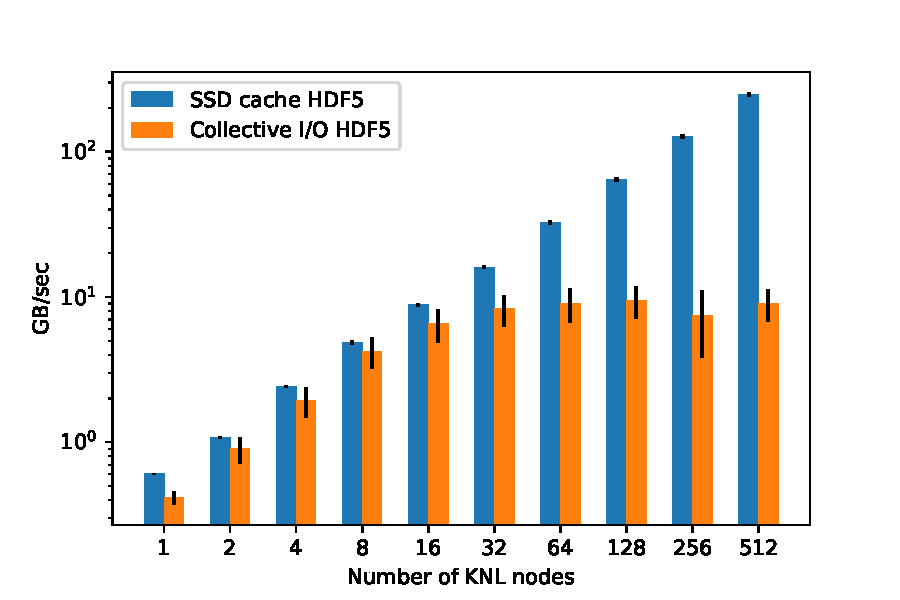
\includegraphics[width=0.6\textwidth]{ssd_cache.pdf}
\caption{HDF5 write rate for collective I/O on Theta Lustre file system. Lustre stripe count is 48, and lustre stripe size is 16MB. The size of the local buffer is 16MB. 32 ranks per node.}\label{fig:perf}
\end{figure}
%\section{Future works}
%\label{sec:future}
%\subsection{Incorporating SSD for repeatedly parallel read}
%Currently, the cache is applied to write only. Local storage can also be used to improve the read performance. This will be particularly useful for repeatedly read applications such as deep learning, where at each epoch, the 
%\subsection{Incorporating the design to the VFD layer}

\subsection{Modification to the HDF5 library}
To incorporate the node-local storage cache functionality into the HDF5 library, we do the following changes to the source code: 
\begin{itemize}
\item Added H5Dio\_cache.c and H5Dio\_cache.h which contains all the *\_cache functions mentioned above.
\item H5Dio.c -- renamed the original H5Dwrite function as H5Dwrite\_direct, and created a new H5Dwrite function which depending on the value of the environmental variable "NODE\_LOCAL\_CACHE", calls either H5Dwrite\_cache or H5Dwrite\_direct. 
\item H5D.c, H5S.c, H5P.c -- modified H5Dclose, H5Sclose, H5Pclose to wait for I/O thread to finish the data migration before closing the dataset object. 
\item H5F.c -- (a) renamed the original H5Fcreate function as H5Fcreate\_direct, and created a new H5Fcreate function which depending on the value of the environmental variable "NODE\_LOCAL\_CACHE", calls either H5Fcreate\_cache or H5Fcreate\_direct. (b) modified H5Fclose to wait for I/O thread to finish the data migration and terminate the I/O thread. 
\end{itemize}

\section{Parallel read workflow}
Previously we have incorporated node-local storage into parallel write, where we write the data to the node-local storage first and then migrate to the file system in the background. Here, we discuss our initial design of incorporating the local storage into read workflow. Again, our goal is to use the local storage as a cache to accelerate the parallel I/O.

The major challenge for read is that, we typically do not know the I/O access pattern before-hand. Therefore, to do data prefetch or cache for very generic application is difficult. We thus start some very common workflow, in particular, for those applications with repeatedly read. We start with deep learning application.
We assume that the dataset is stored in a one HDF5 file with the following organization: dataset.shape = (nsample, sample.shape), where sample.shape is the shape for each individual sample. Nsample is the total number of samples in the dataset. During the training, the application sweeps through the entire dataset multiple times, once per epoch. In each epoch, the samples are read in a batch by batch one-the- fly fashion. The dataset sometimes is also shuffled before the starting of new epoch.
\begin{lstlisting}
for (epoch) { # the application sweep through the entire dataset once per epoch
	for (steps) {# each step, it reads one batch of samples from the dataset. 
		H5_hyperslab_selection(fspace...) # selection by points 
		...
		H5_hyperslab_selection(fspace...)
		H5Dread( ... fspace, ...buf)
		... compute work for processing the batch - forward pass + backward pass ... 
	}
}
\end{lstlisting}
\subsection{Design}
To incorporate the node-local storage into the workflow, we do the following:
In first iteration, we read the dataset from the file system, and then write it to the local storage asynchronously. “Asynchronously” means we create an I/O pthread to perform the writing. The application can continue the training phase. Therefore, this asynchronous write does not introduce any overhead except occupying some resources from the host device. At second iteration, at each read, we will check whether the data is on the local storage or not. If yes, we directly read it from the local storage; otherwise, we will go to the file system to get the data. In order to take care of the data shuffling, we create memory buffer which mapped to the files on the local storage. When then create an MPI\_Win so that all the ranks can access data remotely. The whole workflow is schematically shown in Fig.~\ref{fig:read}. 
\begin{figure}[hbt]
\centering
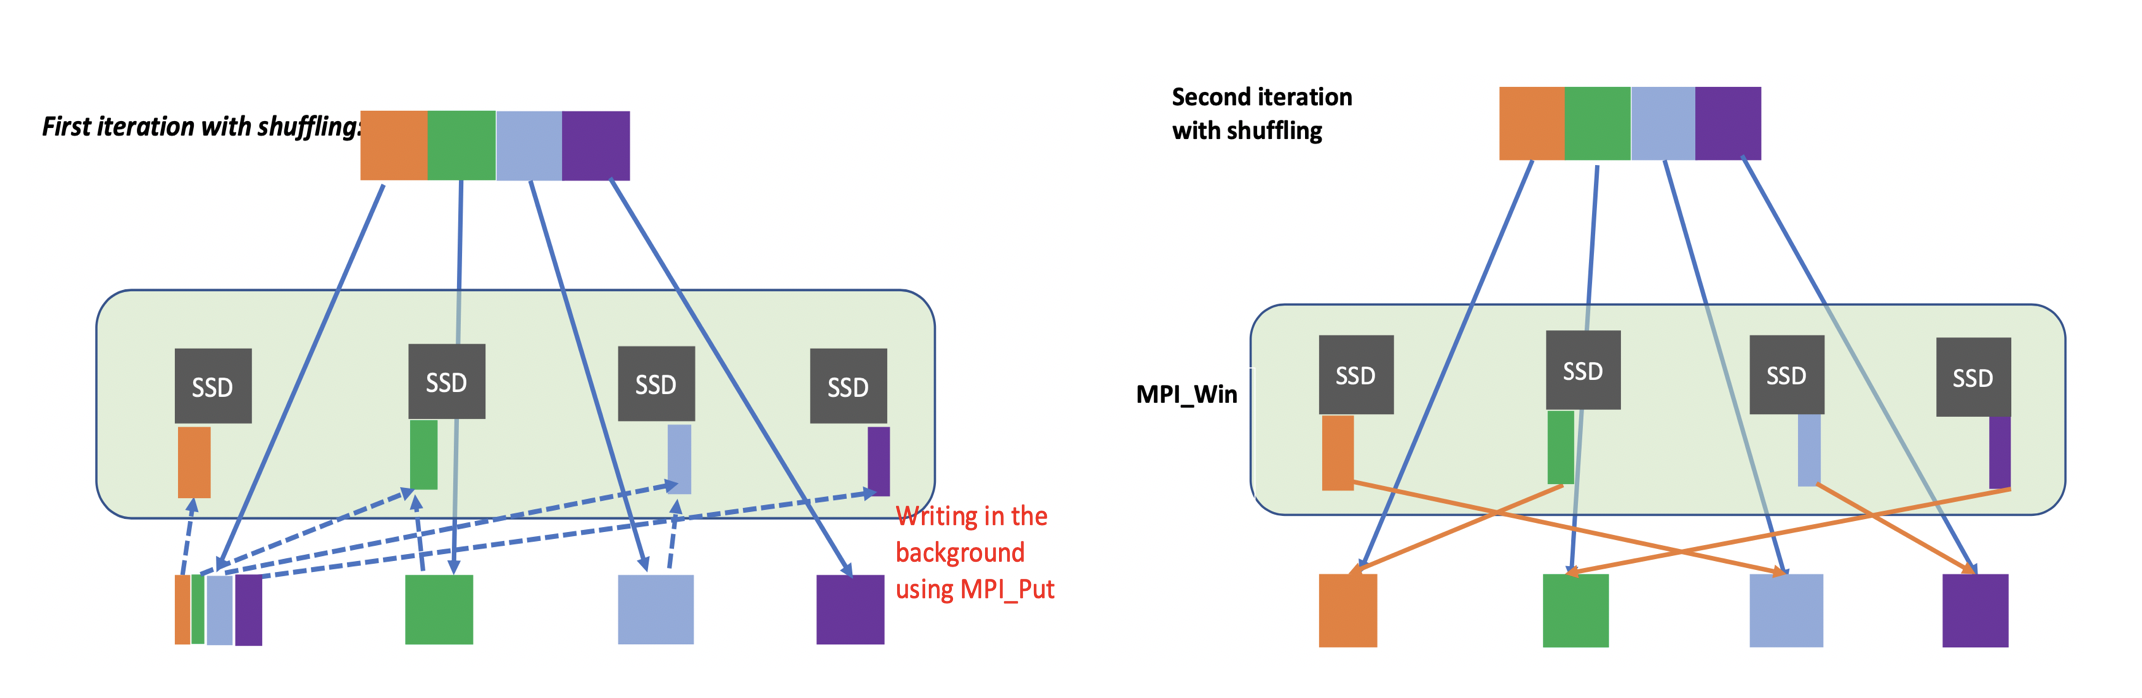
\includegraphics[width=0.9\textwidth]{parallel_read.png}
\caption{Incorporating node-local storage into parallel read workflow. In the first iteration, the data is read from the parallel file system and cached to the node-local storage in asynchronously. In the following up iterations, the data is directly fetch from node-local storage without going to the remote file system. Memory map is created for all the cache files on the node-local storage and attached to an MPI window. The data caching in the first iteration and data fetching in the following up iterations are performed through one-sided RMA. If the data can not fit into the node-local storage entirely, we will have some data left on the filesystem. In this case, we create another MPI window on the parallel file system, and fetch the rest of the data there.}\label{fig:read}
\end{figure}

\subsection{Function APIs}
The major functions exposed to the users are: 
\begin{itemize}
\item H5Dread\_to\_cache -- reading data from the parallel file system and write the buffer to the local storage
\item H5Dread\_from\_cache -- reading data directly from the local storage
\end{itemize}
\subsection{Initial performance evaluation}
The initial performance evaluation is shown in Fig.~\ref{fig:perf_read}. As one can see, with incorporating SSD as a cache, the read performance scales very well and surpass the the Lustre read performance. 
\begin{figure}[hbt]
\centering
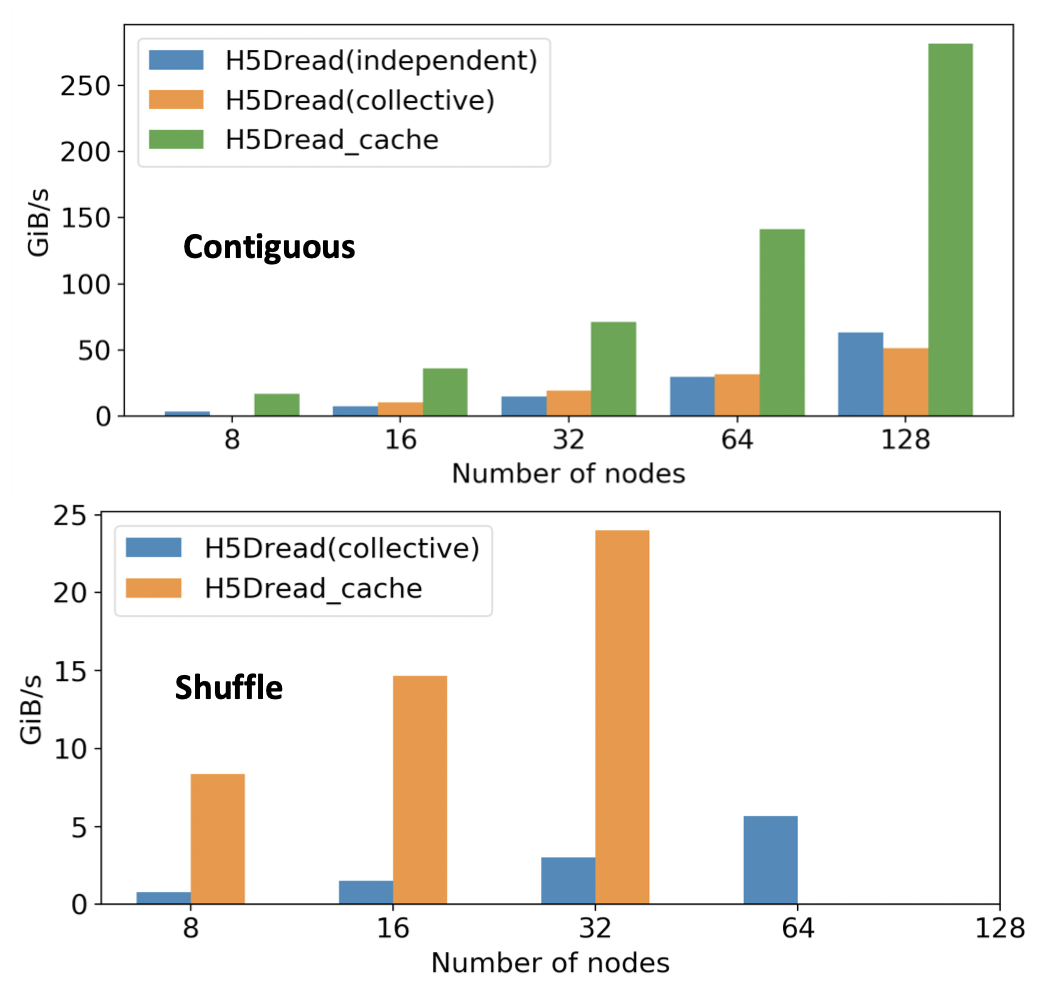
\includegraphics[width=0.6\textwidth]{perf_read.png}
\caption{Scaling of H5Dread with local storage cache in comparison with original H5Dread. We set 1 rank per node in the benchmark.}\label{fig:perf_read}
\end{figure}
\section{Conclusion}
We have demonstrated a prototype implementation that incorporating node-local storage into the I/O workflow by first writing the data to local storage and then migrate the data asynchronously to the file system through an I/O helper pthread. This effectively reduces the I/O cost appeared in the application and hide the data migration in the compute. Our initial performance evaluation has validated the async I/O feature of this implementation and shown that it can achieve an aggregate effective I/O bandwidth much higher than the peak of the file system. The framework and API are designed in a way that makes the whole framework easy to be adopted by the application developers. 
\section*{Acknowledgment}
This research used resources of the Argonne Leadership Computing Facility, which is a DOE Office of Science User Facility supported under Contract DE-AC02-06CH11357.
\end{document}